\documentclass[a4paper,12pt]{article}
\usepackage{graphicx, float, enumerate, parskip}
\usepackage[indonesian]{babel}
\usepackage{amsmath, amsthm, amssymb, amsfonts}
\usepackage{listings, fancyvrb, xcolor}
\usepackage{verbatim}

\theoremstyle{definition}
\newtheorem{definition}{Definisi}[section]
\newtheorem{theorem}{Teorema}[section]
\newtheorem{example}{Contoh}[section]
\lstset{% setup listings
    language=R,% set programming language
    frame=tb,
    basicstyle=\ttfamily\small,% basic font style
    keywordstyle=\color{blue},% keyword style
    commentstyle=\color{gray},% comment style
    breaklines=true,% automatic line breaking
    fancyvrb=true,% verbatim code is typset by listings
}
\usepackage[
    backend=biber,
    style=bwl-FU,
    sorting=nyt,
    maxbibnames=99,
    natbib=true,
]
{biblatex}
\addbibresource{DPustaka.bib}
\usepackage[
    pdfusetitle,
    colorlinks=true,
    linktoc=page,
    allcolors=blue
]{hyperref}

%% ---------------------------
\begin{document}
    \title{Visualisasi dari Data Multivariate}
    \author{Yudha Setya Wicaksana 4112321012\\
    Muthia Yulisa 4112321035}
\date{\today}
\begin{titlepage}
    \maketitle
\end{titlepage}

\section{Plot Kontur}
Sebuah kontur plot merepresentasikan permukaan 3D $(x, y, f(x, y))$ di bidang dengan memproyeksikan kurva level $s f(x, y) = c$ dengan konstant terpilih $c$. Fungsi kontur (\texttt{graphic}) dan kontur plot (\texttt{lattice}) memproduksi kontur plot. Fungsi berisi kontur di graphic package dan levelplot. fungsi dalam paket lattice menghasilkan plot kontur yang terisi. Kedua kontur dan kontur plot memberi label kontur secara default. Variasi dari jenis ini plot adalah gambar (grafik), yang menggunakan warna untuk mengidentifikasi tingkat kontur.

\begin{example}(Contour Plot)

Sebuah contoh disediakan di R menggunakan data gunung api. Informasi tentang data ini ada di file bantuan untuk gunung berapi, Data berupa matriks berukuran 87 x 61 yang berisi informasi topografi untuk Gunung berapi Maunga Whau.

\begin{lstlisting}
# Contour plot with label
contour(volcano, asp=1,labcex=1)

# Packages Lattice
library(lattice)
\end{lstlisting}

Menarik juga untuk melihat permukaan 3D gunung berapi untuk dibandingkan dengan plot kontur. Tampilan 3D dari permukaan gunung berapi disediakan dalam contoh fungsi perspektif plot. Kode R untuk contoh ada di halaman bantuan pers.Untuk run the example, ketikkan \texttt{example(persp)}. 

Jika \texttt{rgl} package sudah terinstall, tampilan 3D interaktif dari gunung berapi muncul dalam contoh. Saat permukaan gunung berapi ditampilkan, gunakan mouse untuk memutar dan memiringkan permukaan, untuk melihatnya dari sudut yang berbeda.

\begin{lstlisting}
library(rgl)
example(rgl)
\end{lstlisting}

Tampilan 3D lain dari data gunung berapi, dengan bayangan untuk menunjukkan kontur level, muncul dalam contoh fungsi \texttt{wireframe} di  kemasan \texttt{lattice}. Lihat contoh pertama di file bantuan wireframe.

\begin{figure}[H]
    \centering
    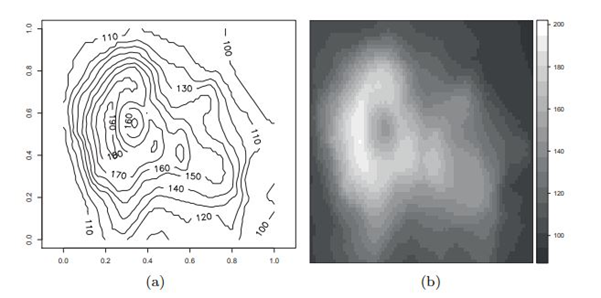
\includegraphics[height=5cm]{gb/K3G1.png}
    \caption{Kontur Plot dan level plot dari data
    gunung berapi pada contoh 5.7 dan 5.8}
    \label{K3G1}
\end{figure}
\end{example}

\begin{example} (konter Plot yang Terisi)

Plot kontur dengan efek 3D bisa jadi ditampilkan dalam 2D dengan melapisi garis kontur pada peta warna yang sesuai ke ketinggian. Fungsi gambar dalam paket grafik menyediakan warna background plot. Plot yang dihasilkan di bawah ini mirip dengan \ref{K3G1}, dengan latar belakang plot dalam warna medan.
\end{example}

\begin{lstlisting}
    image(volcano, col = terrain.colors(100), axes = FALSE)
    contour(volcano, levels = seq(100,200,by = 10), add = TRUE)
\end{lstlisting}

Menggunakan gambar tanpa kontur pada dasarnya menghasilkan jenis plot yang sama Filled.contour (graphic) dan levelplot (lattice). Kontur dari fill.contour dan levelplot diidentifikasikan dengan sebuah legenda daripada melapiskan garis kontur. Bandingkan plot yang dihasilkan oleh gambar dengan mengikuti dua plot.

\begin{lstlisting}
    filled.contour(volcano, color = terrain.colors, asp = 1)
    levelplot(volcano, scales = list(draw = FALSE),
         xlab = "", ylab = "")
\end{lstlisting}

Plot yang dihasilkan oleh levelplot ditunjukkan pada Figure 5.8(b). (Tampilan aktif layar akan berwarna.)

Keterbatasan sebar 2D adalah bahwa untuk kumpulan data besar, sering ada daerah yang datanya sangat padat, dan daerah di mana datanya cukup jarang. Pada kasus ini, scatterplot 2D tidak mengungkapkan banyak informasi tentang kepadatan bivariat. Pendekatan lain adalah menghasilkan histogram 2D atau datar, dengan perkiraan kepadatan di setiap nampan yang diwakili oleh warna yang sesuai.

\begin{example} (2D Histogram)

    Pada contoh ini, simulasi normal bivariat data ditampilkan dalam histogram datar dengan nampan heksagonal. Fungsi heksbin dalam paket hexbin (tersedia dari repositori Biokonduktor) menghasilkan sebuah versi dasar plot ini dalam skala abu-abu, ditunjukkan pada Gambar 2

\begin{lstlisting}
    library(hexbin)
    x <- matrix(rnorm(4000), 2000, 2)
    plot(hexbin(x[,1], x[,2]))
\end{lstlisting}

Bandingkan histogram kerapatan rata pada Gambar 2 dengan histogram bivariat.Pada Gambar 12.11. Perhatikan bahwa warna yang lebih gelap sesuai dengan wilayah tempat kepadatan tertinggi, dan warna semakin terang di sepanjang garis radial memanjang dari modus dekat titik asal. Plot menunjukkan kira-kira simetri melingkar, konsisten dengan densitas normal bivariat standar.

Histogram bivariat juga dapat ditampilkan dalam 2D menggunakan palet warna, seperti heat.colors atau terrain.colors, untuk mewakili kerapatan masing-masing bin.

Versi ggplot dari histogram 2D hexbin dapat ditampilkan menggunakan geomhex, Argumen pertama untuk ggplot harus berupa kerangka data.

\begin{lstlisting}
    library(ggplot2)
    x <- data.frame(x)
    ggplot(x, aes(x[,1], x[,2])) + geom_hex()
\end{lstlisting}

Angka yang dihasilkan (tidak ditampilkan) sangat mirip dengan Gambar 12.11, tetapi dalam warna.

Jenis plot serupa diimplementasikan dalam paket gplots. Itu plot (tidak ditampilkan) yang dihasilkan dari kode berikut mirip dengan Gambar 2, tetapi dengan tempat sampah warna dan persegi.

\begin{lstlisting}
    library(gplots)
    hist2d(x, nbins = 30,
      col = c("white", rev(terrain.colors(30))))
\end{lstlisting}

\begin{figure} [H]
    \centering
    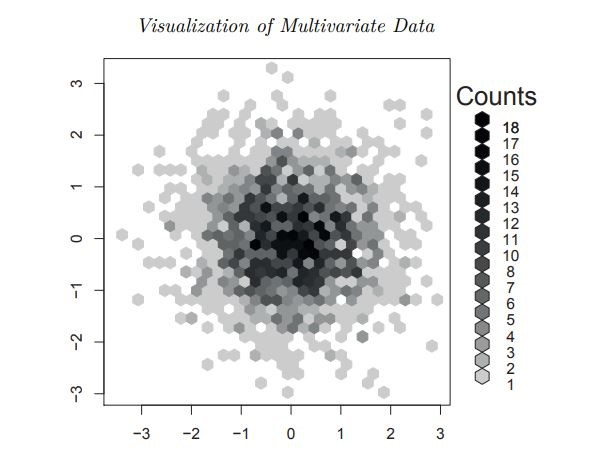
\includegraphics[height=5cm]{gb/K3G2.jpg}
    \caption{Histogram densitas rata dari data normal bivariat dengan nampan heksagonal yang dihasilkan oleh hexbin pada Contoh 1.3.}
    \label{fig:my_label}
\end{figure}
\end{example}

\section{Representasi Data 2D Lain}
Selain plot kontur dan proyeksi data lainnya menjadi dua dimensi, ada beberapa metode lain untuk merepresentasikan data multivariat dalam dua dimensi. Ini termasuk, antara lain, kurva Andrews, plot koordinat paralel, dan berbagai tampilan ikonografi seperti plot segmen dan star plot.

\subsection{Andrews Curves}
Jika $X_1, . . . , X_n \in\mathbb{R}^d$, salah satu pendekatan untuk memvisualisasikan data dalam dua dimensi adalah dengan memetakan masing-masing vektor data sampel ke fungsi bernilai nyata. Kurva Andrews memetakan setiap pengamatan sampel $x_i = x_{i1}, . . . , x_{id}$ ke sebuah fungsi.

\begin{equation*}
f_i(t)=\frac{x_i1}{\sqrt{2}}+x_{i_2} \sin t+ x_{i_3} \cos t+ x_{i_4} \sin 2t+ x_{i_5} sin 2t+...
\end{equation*}

\begin{equation*}
= \frac{x_{i_1}}{\sqrt{2}} + \sum_{1\leq k\leq d/2} x_i, _{2k} sin kt + \sum_{1\leq k < d/2} x_i,_{2k+1} cos kt, -\pi \leq t\leq \pi 
\end{equation*}

Dengan demikian, setiap pengamatan diwakili oleh proyeksi ke satu set fungsi basis orthogonal      . Perhatikan bahwa perbedaan antara pengukuran lebih diperkuat dalam istilah frekuensi yang lebih rendah, jadi bahwa representasi tergantung pada urutan variabel atau fitur.

\begin{example} (Kurva Andrews)

Dalam contoh ini, pengukuran daun diambil di N. Queensland, Australia untuk dua tipe arsitektur daun \cite{King1999} adalah diwakili oleh kurva Andrews. Kumpulan data leafshape17 dalam DAAG paket [189,190]. Tiga pengukuran (panjang daun, tangkai daun, dan lebar daun) sesuai dengan titik-titik di R3. Paling mudah untuk menginterpretasikan plot jika arsitektur daun diidentifikasi dengan warna yang berbeda, tetapi di sini kami menggunakan jenis garis yang berbeda. Untuk memplot kurva, tentukan fungsi untuk menghitung $f_i(t)$ untuk titik arbitrer $x_i$ di dalam R3 dan $-\pi\leq t\leq \pi $. Evaluasi fungsi sepanjang interval $[-\pi,\pi]$ untuk masing-masing titik sampel $x_i$.

\begin{lstlisting}
    library(DAAG)
    attach(leafshape17)
    f <- function(a, v) {
    #Andrews curve f(a) for a data vector v in R^3
    v[1]/sqrt(2) + v[2]*sin(a) + v[3]*cos(a)
    }
    #scale data to range [-1, 1]
    x <- cbind(bladelen, petiole, bladewid)
    n <- nrow(x)
    mins <- apply(x, 2, min) #column minimums
    maxs <- apply(x, 2, max) #column maximums
    r <- maxs - mins #column ranges
    y <- sweep(x, 2, mins) #subtract column mins
    y <- sweep(y, 2, r, "/") #divide by range
    x <- 2 * y - 1 #now has range [-1, 1]
    #set up plot window, but plot nothing yet
    plot(0, 0, xlim = c(-pi, pi), ylim = c(-3,3),
    xlab = "t", ylab = "Andrews Curves",
    main = "", type = "n")
    #now add the Andrews curves for each observation
    #line type corresponds to leaf architecture
    #0=orthotropic, 1=plagiotropic
    a <- seq(-pi, pi, len=101)
    dim(a) <- length(a)
    for (i in 1:n) {
    g <- arch[i] + 1
    y <- apply(a, MARGIN = 1, FUN = f, v = x[i,])
    lines(a, y, lty = g)
    }
    legend(3, c("Orthotropic", "Plagiotropic"), lty = 1:2)
    detach(leafshape17)
\end{lstlisting}

Plot kurva Andrews untuk contoh ini ditunjukkan pada Gambar 5.10. Plot tersebut menjelaskan kesamaan dalam arsitektur daun plagiotropik dan ortotropik kelompok, dan perbedaan antara kelompok-kelompok ini. Secara umum, jenis plot ini mungkin mengungkapkan kemungkinan pengelompokan data.
\end{example}

R note 5.3
Dalam Contoh 5.10 operator sapuan diterapkan untuk mengurangi kolom minimum di atas Sintaxnya adalah.

\begin{lstlisting}
    sweep(x, MARGIN, STATS, FUN="-", ...)
\end{lstlisting}

Secara default, statistik dikurangi tetapi operasi lain dimungkinkan. di Sini 

\begin{lstlisting}
    y <- sweep(x, 2, mins) #subtract column mins
    y <- sweep(y, 2, r, "/") #divide by range
\end{lstlisting}

Menyapu (mengurangi) minimum setiap kolom (margin = 2). Kemudian rentang masing-masing dari tiga kolom (dalam r) disapu; itu adalah, setiap kolom dibagi dengan jangkauannya.


\subsection{Plot Koordinat Paralel}

Plot koordinat paralel memberikan pendekatan lain untuk visualisasi data multivariat. Representasi vektor dengan koordinat paralel diperkenalkan oleh \cite{Inselberg1985} dan diterapkan untuk analisis data oleh \cite{Wegman1990}. Selain merepresentasikan sumbu sebagai ortogonal, sistem koordinat paralel merepresentasikan sumbu sebagai garis paralel berjarak sama. Biasanya garis-garis ini horizontal dengan asal, skala, dan orientasi yang sama. Kemudian untuk mewakili vektor dalam R d, koordinat paralel hanyalah koordinat sepanjang d salinan dari garis nyata. Setiap koordinat vektor kemudian diplot sepanjang korespondensinya sumbu, dan titik-titik tersebut digabungkan dengan ruas garis.

Plot koordinat paralel diimplementasikan oleh fungsi parcoord di Paket MASS [293] dan fungsi paralel dalam paket kisi [257]. Fungsi parcoord menampilkan sumbu sebagai garis vertikal. Fungsi panel paralel menampilkan sumbu sebagai garis horizontal.

\begin{example} (Koordinat Paralel)

    Contoh ini mengilustrasikan menggunakan fungsi paralel (lattice) untuk membuat tampilan panel plot koordinat paralel untuk data crabs (MASS) [293]. Kerangka data kepiting memiliki 5 pengukuran pada masing-masing 200 kepiting, dari empat kelompok ukuran 50. Kelompok diidentifikasi berdasarkan spesies (biru atau jingga) dan jenis kelamin. Grafik paling baik dilihat dalam warna. Di sini kami menggunakan hitam dan putih, dan untuk keterbacaan pilih hanya 1/5 dari data.

    \begin{lstlisting}
        library(MASS)
        library(lattice)
        #trellis.device(color = FALSE) #black and white display
        x <- crabs[seq(5, 200, 5), ] #get every fifth obs.
        parallelplot(~x[4:8] | sp*sex, x)
    \end{lstlisting}

    Plot koordinat paralel yang dihasilkan ditampilkan pada Gambar 5.11(a) label sepanjang sumbu vertikal mengidentifikasi setiap sumbu yang sesuai dengan lima pengukuran (ukuran lobus frontal, lebar belakang, panjang karapas, lebar karapas, tubuh,kedalaman). Sebagian besar variabilitas antar kelompok dalam ukuran keseluruhan. Menyesuaikan pengukuran ukuran masing-masing kepiting dapat menghasilkan lebih banyak plot yang menarik. Mengikuti saran dalam Venables dan Ripley [293], kami sesuaikan pengukuran dengan luas karapas.

    \begin{lstlisting}
        #trellis.device(color = FALSE) #black and white display
        x <- crabs[seq(5, 200, 5), ] #get every fifth obs.
        a <- x$CW * x$CL #area of carapace
        x[4:8] <- x[4:8] / sqrt(a) #adjust for size
        parallelplot(~x[4:8] | sp*sex, x)
    \end{lstlisting}

    Dalam plot yang dihasilkan pada Gambar 5.11(b), terdapat banyak perbedaan spesies dan jenis kelamin lebih jelas setelah penyesuaian daripada di Gambar 5.11(a).

    \begin{figure} [H]
        \centering
        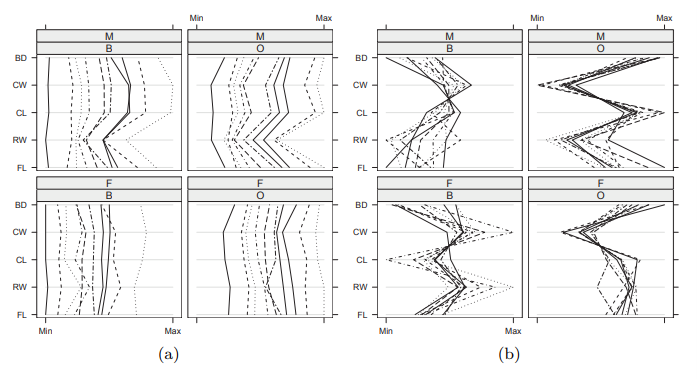
\includegraphics[height=5cm]{gb/K3G3.png}
        \caption{Plot koordinat paralel pada Contoh 5.11 untuk subhimpunan dari data kepiting (MASS). (a) Perbedaan antara spesies (B=biru, O=oranye) dan jenis kelamin (M, F) sebagian besar dikaburkan oleh variasi besar dalam ukuran keseluruhan. (b) Setelah menyesuaikan pengukuran untuk ukuran masing-masing kepiting, perbedaan antara kelompok terlihat jelas.}
        \label{fig:my_label}
    \end{figure}
\end{example}

\subsection{Segmen, Bintang, dan Representasi Lainnya}

Data multivariat dapat diwakili oleh ikon dua dimensi atau mesin terbang, seperti bintang. Kurva Andrews pada Contoh 5.10 adalah contohnya; itu kurva adalah simbol dua dimensi. Kurva Andrews ditampilkan ditumpangkan pada sistem koordinat yang sama. Representasi lain sebagai ikon adalah paling baik ditampilkan dalam tabel, sehingga ciri-ciri pengamatan dapat dibandingkan. Tampilan tabular tidak memiliki banyak nilai praktis untuk dimensi tinggi atau set data besar, tetapi dapat berguna untuk beberapa set data kecil. Beberapa contoh termasuk plot bintang dan plot segmen. Jenis plot ini mudah diperoleh di R menggunakan fungsi bintang (grafik). 

\begin{example}(Segmen Plot)

    Contoh ini menggunakan subset dari kepiting (MASS) data dari Contoh 5.11. Seperti pada Contoh 5.11, pengukuran individu disesuaikan dengan ukuran keseluruhan berdasarkan luas karapas.

    \begin{lstlisting}
        #segment plot
        x <- MASS::crabs[seq(5, 200, 5), ] #get every fifth obs.
        x <- subset(x, sex == "M") #keep just the males
        a <- x$CW * x$CL #area of carapace
        x[4:8] <- x[4:8] / sqrt(a) #adjust for size
        
        #use default color palette or other colors
        #palette(gray(seq(.4, .95, len = 5))) #use gray scale
        palette(rainbow(6)) #or use color
        stars(x[4:8], draw.segments = TRUE,
        labels =levels(x$sp), nrow = 4,
        ylim = c(-2,10), key.loc = c(3,-1))
        
        #after viewing, restore the default colors
        palette("default")
    \end{lstlisting}

    Plotnya ditunjukkan pada Gambar 5.12. Pengamatan diberi label oleh spesies. Itu perbedaan antara spesies (untuk jantan) dalam sampel ini cukup jelas pada plot. Plot menunjukkan, misalnya, bahwa kepiting oranye memiliki tubuh yang lebih besar kedalaman relatif terhadap lebar karapas daripada kepiting biru.

    \begin{figure}[H]
        \centering
        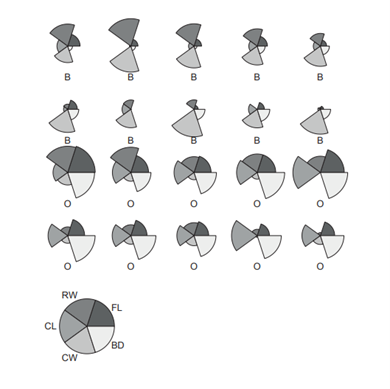
\includegraphics[height=7cm]{gb/K3G4.png}
        \caption{Plot segmen subset jantan dalam kepiting (MASS)  kumpulan data pada Contoh 5.12. Pengukuran telah disesuaikan secara keseluruhan ukuran individu kepiting. Kedua spesies tersebut berwarna biru (B) dan jingga (O).}
        \label{fig:my_label}
    \end{figure}
\end{example}

\section{Analisis Komponen Utama}

  Analisis komponen utama (PCA) mengacu pada pengurangan dimensi metode. Kumpulan data mungkin memiliki sejumlah besar variabel berkorelasi, dan PCA adalah metode yang memberikan representasi perkiraan dalam bentuk yang lebih rendah ruang dimensi. Di bagian ini, kami meninjau bagaimana PCA digunakan untuk membantu memvisualisasikan dan menjelajahi data multivarian. Ini memiliki banyak aplikasi lain, seperti regresi komponen utama, dalam supervised learning, dan dalam unsupervised learning.

  Analisis komponen utama untuk visualisasi multivariat menggunakan proyeksi (lihat, misalnya, [194, Bab 8] dan [293, Bagian 11.1]). Ketika data diproyeksikan ke vektor eigen yang sesuai dengan nilai eigen maksimal dari matriks kovarians, komponen utama pertama ini berada di arah yang menjelaskan variasi data yang paling banyak. Dimensi dikurangi dengan memproyeksikan ke a sejumlah kecil komponen utama yang secara kolektif menjelaskan sebagian besar variasi. 

Contoh 5.13

(PCA untuk ujian buku terbuka dan tertutup). Skor (bootstrap) data (dibahas dalam [194]) memiliki nilai ujian dalam lima mata pelajaran: mekanika, vektor, aljabar, analisis, dan statistik, untuk 88 siswa. Mekanika dan vektor adalah buku tertutup, dan tiga ujian lainnya adalah open book.

 Sebagai langkah pertama dalam analisis data, kita mungkin melihat plot pencar berpasangan dan korelasi berpasangan antar variabel. Jelas bahwa beberapa dari variabel tersebut sangat berkorelasi. Dengan PCA kita dapat menghitung turunan variabel yang meringkas data dalam sistem koordinat lain menggunakan variabel yang tidak berkorelasi, kemungkinan menangkap sebagian besar hubungan dalam dua atautiga komponen. Orang mungkin menyelidiki apakah dua komponen utama pertama adalah representasi data yang memadai dalam dua dimensi, dan terapkan hasilnya untuk visualisasi data yang lebih baik.

 \begin{lstlisting}
library(bootstrap)
str(scor)
pairs(scor)
cor(scor)
\end{lstlisting}

\begin{verbatim}
mec vec alg ana sta
mec 1.0000000 0.5534052 0.5467511 0.4093920 0.3890993
vec 0.5534052 1.0000000 0.6096447 0.4850813 0.4364487
alg 0.5467511 0.6096447 1.0000000 0.7108059 0.6647357
ana 0.4093920 0.4850813 0.7108059 1.0000000 0.6071743
sta 0.3890993 0.4364487 0.6647357 0.6071743 1.0000000    
\end{verbatim}

 

 Rincian berikut mengilustrasikan perhitungan aljabar linier yang diperlukan untuk menurunkan komponen utama. Kemudian kami membandingkan hasil ini dengan fungsi prcomp pada data yang sama. Langkah pertama dalam PCA adalah menghitung dekomposisi spektral dari matriks kovarians dari data yang dipusatkan dan diskalakan untuk mendapatkan nilai eigen dan vektor eigen.

 \begin{lstlisting}
     n <- nrow(scor)
x <- scale(scor) #center and scale
s <- cov(x)
e <- eigen(s)
lam <- e$values #vector of eigenvalues
P <- e$vectors #matrix of eigenvectors
 \end{lstlisting}

 Screeplot membantu menentukan berapa banyak akun komponen utama untuk sebagian besar varian. Dua versi, plot garis dan plot bar diberikan di bawah. Plot garis ditunjukkan pada Gambar 5.13. Proporsi varians dan proporsi varians kumulatif yang dijelaskan untuk setiap komponen utama dirangkum dalam tabel. Bandingkan proporsi kumulatif dengan merencanakan; plot nilai eigen diratakan ketika persentasenya mendekati 90%.

 \begin{figure}
     \centering
     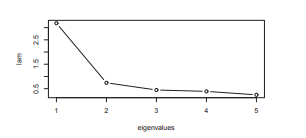
\includegraphics{{gb/gambar 5.13.png}}
     \caption{GAMBAR 5.13: Screeplot (nilai eigen) untuk data skor pada 5.13.}
     \label{fig:my_label}
 \end{figure} {H}
 \begin{lstlisting}
     plot(lam, type = "b", xlab = "eigenvalues", main = "")
barplot(lam, xlab = "eigenvalues")
tab <- rbind(lam / sum(lam), cumsum(lam) / sum(lam))
> tab
[,1] [,2] [,3] [,4] [,5]
[1,] 0.636196 0.1479144 0.08899303 0.07757848 0.0493181
[2,] 0.636196 0.7841104 0.87310342 0.95068190 1.0000000
 \end{lstlisting}

 Plot dan tabel menunjukkan bahwa tiga PC dapat memberikan hasil yang memadai representasi data. Untuk dua PC sekitar 78 % dari total varian ditangkap, yang meningkat menjadi 87% untuk tiga PC. Untuk menerjemahkan persamaan  ke dalam bentuk matriks, misalkan X adalah matriks data yang terpusat dan diskalakan dan P adalah matriks standar vektor eigen dari Cov(Σ) ˆ . Maka Z = XP.

 \begin{lstlisting}
     ## x is already centered and scaled above
z <- x %*% P
> dim(z)
[1] 88 5
> head(z)
[,1] [,2] [,3] [,4] [,5]
1 -4.285041 0.67410225 0.1235891 0.7931108 -0.51438033
2 -4.541989 -0.21331176 -0.2317797 0.5516063 0.59618974
3 -4.102690 0.27557530 0.5304377 0.6096862 -0.02781595
4 -3.026846 -0.14916207 -0.3702154 0.1595890 -0.43950477
5 -2.882081 -0.04408014 0.2988861 -0.3225740 -0.14767795
6 -2.988775 -0.68126196 0.2628756 0.2950331 0.54754485

 \end{lstlisting}

 Bagian atas matriks Z ditunjukkan di atas. Kelima kolom tersebut adalah lima pokok komponen untuk enam pengamatan pertama. R menyediakan fungsi princomp dan prcomp yang menghitung komponen utama. Pemuatan dikembalikan dalam komponen rotasi prcomp atau komponen loading princomp.

 \begin{lstlisting}
  pc <- prcomp(scor, center = TRUE, scale = TRUE)
> summary(pc)
Importance of components:
PC1 PC2 PC3 PC4 PC5
Standard deviation 1.7835 0.8600 0.66706 0.62281 0.49658
Proportion of Variance 0.6362 0.1479 0.08899 0.07758 0.04932
Cumulative Proportion 0.6362 0.7841 0.87310 0.95068 1.00000   
 \end{lstlisting}

 Dalam tabel ringkasan untuk hasil prcomp, proporsi varians dijelaskan oleh masing-masing PC, serta proporsi kumulatifnya, cocokkan dengan tabel kami  dihitung dari nilai eigen. Metode prediksi diterapkan di bawah ini untuk lima nilai ujian pertama. Itu hasilnya sama dengan lima baris pertama matriks PC z yang dihitung di atas.

 \begin{lstlisting}
     > df <- scor[1:5, ]
> predict(pc, newdata = df) #same as z above
PC1 PC2 PC3 PC4 PC5
1 -4.285041 -0.67410225 0.1235891 0.7931108 -0.51438033
2 -4.541989 0.21331176 -0.2317797 0.5516063 0.59618974
3 -4.102690 -0.27557530 0.5304377 0.6096862 -0.02781595
4 -3.026846 0.14916207 -0.3702154 0.1595890 -0.43950477
5 -2.882081 0.04408014 0.2988861 -0.3225740 -0.14767795

 \end{lstlisting}

 
Prediksi juga dapat ditemukan dari prcomp menggunakan komponen rotasi.

\begin{lstlisting}
    > head(x %*% pc$rotation, 5)
PC1 PC2 PC3 PC4 PC5
1 -4.285041 -0.67410225 0.1235891 0.7931108 -0.51438033
2 -4.541989 0.21331176 -0.2317797 0.5516063 0.59618974
3 -4.102690 -0.27557530 0.5304377 0.6096862 -0.02781595
4 -3.026846 0.14916207 -0.3702154 0.1595890 -0.43950477
5 -2.882081 0.04408014 0.2988861 -0.3225740 -0.14767795

\end{lstlisting}

Bandingkan vektor eigen P dan matriks rotasi komponen utama. Mereka identik kecuali untuk kemungkinan perbedaan tanda vektor eigen dan PC, karena vektor eigen dari matriks kovarian hanya unik hingga tanda mereka.

\begin{lstlisting}
    head(P)
head(pc$rotation)

\end{lstlisting}

Lihat contoh berikut untuk pembahasan lebih lanjut

Contoh 5.14 (PC Biplot). Metode biplot untuk prcomp atau princomp objek adalah sebidang data dalam sistem koordinat dari dua PC pertama. Ini jenis plot dapat membantu untuk visualisasi data dalam dimensi rendah ruang dan untuk interpretasi komponen. Metode biplot bersifat umum,dan biplot PC bukan default. Untuk mendapatkan biplot PC, tentukan pc.biplot = BENAR. Berikut ini lanjutan Contoh 5.13.

\begin{lstlisting}
    ## plot scor data in the (PC1, PC2) coordinate system
biplot(pc, pc.biplot = TRUE)

\end{lstlisting}

Biplot memberikan tampilan baru dari data dimensional skor di (Z1, Z2) pesawat. Bandingkan titik berlabel di biplot dengan Zj/$ \sqrt{\lambda }j$ untuk memahami plotnya.
Dari biplot pada Gambar 5.14, terlihat beberapa wawasan. Aljabar merah vektor memiliki kemiringan hampir nol sehubungan dengan PC kedua; ini menunjukkan bahwa aljabar hanya berbobot ringan di PC2. Kami juga dapat mengamati statistik itu dan skor analisis memiliki bobot positif pada PC2, sedangkan mekanika dan vector memiliki bobot negatif pada arah PC2. Ini dikonfirmasi dalam rotasi matriks, dengan melihat tanda-tanda pada dua kolom pertama. Perhatikan juga itu aljabar memiliki pemuatan tertinggi di PC5.PCA juga dapat diartikan dengan melihat tabel korelasi PC dengan variabel asli.

\begin{lstlisting}
    > round(cor(x, z), 3)
[,1] [,2] [,3] [,4] [,5]
mec -0.713 0.555 0.414 -0.091 -0.065
vec -0.769 0.380 -0.470 0.186 -0.090
alg -0.898 -0.111 -0.025 -0.068 0.420
ana -0.815 -0.334 -0.091 -0.415 -0.210
sta -0.782 -0.405 0.208 0.410 -0.116
\end{lstlisting}

Tabel korelasi menunjukkan variabel yang memiliki korelasi kuat dengan baik PC1 maupun PC2 sama-sama mec dan sta, padahal kelimanya sama-sama kuat.korelasi dengan PC1. PC5 mewakili kurang dari 5% dari total varians; dia terutama berbobot pada skor aljabar. Ujian buku tertutup adalah mekanika dan vektor. Dua PC pertama bobot keduanya positif, tetapi bobot ujian buku terbuka berlawanan tanda-tanda. Hal sebaliknya terjadi pada tabel korelasi.

\begin{figure} {H}
    \centering
    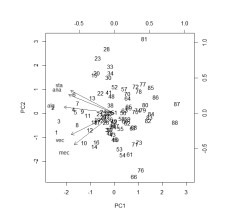
\includegraphics{gb/gambar 5.14.jpg}
    \caption{GAMBAR 5.14: Biplot komponen utama untuk data skor pada 5.14.}
    \label{fig:my_label}
\end{figure}

Contoh 5.15 (data dasalomba). 

Lihat data decathlon (FactoMineR paket, [178]) diperkenalkan pada Contoh 5.2. Berdasarkan plot korelasi, kita mungkin berharap bahwa analisis komponen utama dapat mencerminkan asosiasi antara kelompok peristiwa lintasan dan kelompok peristiwa lapangan. Penampilan pengukuran bervariasi dalam skala, jadi kami ingin menggunakan matriks korelasi dari matriks kovarians untuk PCA.

\begin{lstlisting}
    library(FactoMineR)
data(decathlon)
pc <- princomp(decathlon[,1:10], cor = TRUE, scores = TRUE)
plot(pc) # screeplot
biplot(pc)
\end{lstlisting}

Ringkasan di bawah ini menunjukkan bahwa hampir 75% varian dijelaskan oleh empat komponen utama pertama dan screeplot dari nilai eigen (tidak ditampilkan) menunjukkan bahwa empat hingga enam PC menangkap sebagian besar varian. Biplot ditunjukkan pada Gambar 5.15.

\begin{lstlisting}
    Importance of components:
Comp.1 Comp.2 Comp.3
Standard deviation 1.8088409 1.3180027 1.1852918
Proportion of Variance 0.3271906 0.1737131 0.1404917
Cumulative Proportion 0.3271906 0.5009037 0.6413953
Comp.4 Comp.5 Comp.6
Standard deviation 1.0280323 0.82751044 0.77412446
Proportion of Variance 0.1056850 0.06847735 0.05992687
Cumulative Proportion 0.7470804 0.81555771 0.87548458
\end{lstlisting}

Meskipun beberapa label diplot secara berlebihan pada Gambar 5.15, salah satunya bisa amati bahwa sumbu untuk bidang event shotput, discus, lempar lembing dan lompat tinggi kira-kira dalam arah yang sama, dan hampir ortogonal ke Panjang melompat. Acara sprint (100 m, 110 m rintangan) hampir sama arahnya dan panjang, dan juga hampir orthogonal terhadap kejadian lapangan. Informasi ini konsisten dengan apa yang kami amati dari plot korelasi pada Contoh 5.2.
\section{  Pendekatan Lain Untuk Visualisasi Data}

Banyak metode lain untuk visualisasi data ada dalam literatur dan kami sebutkan di sini hanya beberapa lagi. Tur akbar Asimov [19] bersifat interaktif alat grafis yang memproyeksikan data ke bidang, berputar melalui semua sudut ke mengungkapkan struktur apa pun dalam data. Paket tourr [316] mengimplementasikan beberapa jenis wisata. Tur akbar mirip dengan eksplorasi pengejaran proyeksi analisis data (PPEDA) (Friedman dan Tukey [103]). Dalam kedua kasus, struktur dapat didefinisikan sebagai penyimpangan dari normalitas. Setelah struktur dihapus, pencarian dapat diulang sampai tidak ada struktur signifikan yang tersisa. Pola pengakuan dan penambangan data adalah dua bidang penelitian luas yang menggunakan beberapa metode visualisasi. Lihat Ripley [235] atau Duda et al. [78].

Paket FactoMineR [178] menampilkan alat khusus untuk analisis dan visualisasi data eksplorasi multivariat, termasuk analisis komponen utama, analisis korespondensi, analisis korespondensi berganda, dananalisis banyak faktor. Kumpulan topik yang menarik tentang penambangan data dan visualisasi data ditemukan di Rao, Wegman, dan Solka [233]. Untuk sebuah sumber yang bagus untuk visualisasi data kategorikal lihat Friendly [105] dan http://www.math.yorku.ca/SCS/vcd/.

 Selain fungsi dan paket R yang disebutkan dalam bab ini, beberapa metode tersedia dalam paket lain. Sekali lagi, di sini kami hanya menyebutkan sedikit. Paket latticeExtra [259] memperluas paket lattice. Mosaik plot untuk visualisasi data kategorikal tersedia di petak mosaik.   

\begin{figure} [H]
    \centering
    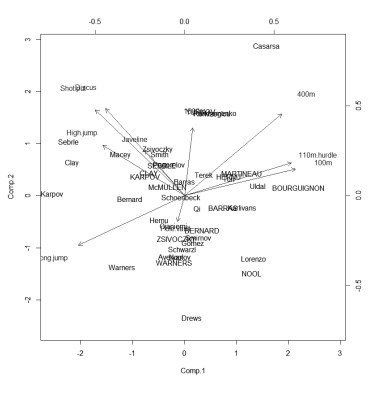
\includegraphics[height=5cm]{gb/gambar 5.15.jpg}
    \caption{GAMBAR 5.15: Biplot komponen utama untuk data decathlon pada 5.15.}
  \label{fig:my_label}
\end{figure}

Lihat paket vcd [208] untuk visualisasi data kategorikal. wajah Chernoff [51] diimplementasikan di wajah (aplpack) [321] dan di wajah (TeachingDemos) [269]. Banyak paket untuk R berada di bawah penambangan data atau pembelajaran mesin payung; sebagai permulaan lihat nnet [293], rpart [283], dan randomForest [184].Lebih banyak paket dijelaskan pada Tampilan Tugas Multivariat dan Mesin Mempelajari Tampilan Tugas di web CRAN.

 Paket rggobi [174] menyediakan antarmuka baris perintah ke GGobi, yang merupakan program visualisasi sumber terbuka untuk menjelajahi dimensi tinggi data. GGobi memiliki antarmuka pengguna grafis, menyediakan dinamis dan interaktif grafis. Perangkat lunak GGobi dapat diperoleh dari http://www.ggobi.org/download/.  Pembaca dirujuk ke dokumentasi dan contoh di http://www.ggobi.org/rggobi. dan buku karya Cook dan Swayne [57] ditampilkan contoh menggunakan R dan GGobi.

 Paket tourr [316] mengimplementasikan metode tur untuk visualisasi data multivariat


\section{Sumber Daya Tambahan}

Paket Cookbook dan gcookbook Chang's R Graphics [46, 47] bagus sumber daya untuk pengguna yang menginginkan contoh yang menunjukkan bagaimana grafik R bisa dikonversi ke grafis ggplot [313]. Murrell [214] mencakup grafis tradisional dalam R, grafik grid, grafik lattice, dan ggplot2. Dokumentasi yang lebih luas disediakan di Wickham [313] untuk ggplot2 dan di Sarkar [258] untuk lattice.

Ada beberapa galeri grafis dan sumber daya yang tersedia secara online mengilustrasikan grafik yang menarik dengan kode R, menampilkan grafik dengan gaya yang bervariasidan kompleksitas,misalnya:

Koleksi umum menggunakan grafik R dan paket lainnya:
\begin{itemize}
\item \url{http://rgraphgallery.blogspot.com/}
\item http://www.r-graph-gallery.com/
\item $http://scs.math.yorku.ca/index.php/R_Graphs_Gallery$
\item http://shinyapps.stat.ubc.ca/r-graph-catalog/
\end{itemize}

Grafik menggunakan ggplot2 atau paket kisi atau ekstensinya:

\begin{itemize}
\item http://www.cookbook-r.com/Graphs/
\item http://www.ggplot2-exts.org/gallery/
\item http://r-statistics.co/Top50-Ggplot2-Visualizations-MasterList-R-Code.html
\item https://plot.ly/ggplot2/
\item http://latticeextra.r-forge.r-project.org/
\end{itemize}

\newpage
\printbibliography[heading=bibintoc,title={Daftar Pustaka}]

\end{document}